\documentclass[12pt]{beamer}
\usepackage[utf8]{inputenc}
\usepackage{amsmath}
\usepackage{amsfonts}
\usepackage{amssymb}
\usepackage{graphicx}
\author{Nico Fröhlich}
\title{NTFS}
\subtitle{New Technology File System}
\subject{IT - Herr Hammer}
\setbeamercolor{background canvas}{bg=black}
\setbeamercolor{normal text}{fg=white}
\setbeamercolor{frametitle}{bg=darkgray}
\setbeamercolor{frametitle}{fg=white}
\setbeamercolor{title}{fg=white}
\setbeamerfont{title}{size=\Huge}
\setbeamerfont{subtitle}{size=\large}
\setbeamerfont{name}{size=\medium}
\setbeamerfont{date}{size=\footnotesize}
\setbeamerfont{normal text}{size=\Huge}
\setbeamerfont{item}{size=\Huge}
\setbeamerfont{item projected}{size=\Huge}
\setbeamerfont{itemize item}{size=\Huge}
\setbeamerfont{itemize subitem}{size=\Huge}
\setbeamerfont{itemize subsubitem}{size=\Huge}
\setbeamerfont{itemize/enumerate body}{size=\Huge}
\setbeamerfont{itemize/enumerate subbody}{size=\Huge}
\setbeamerfont{itemize/enumerate subsubbody}{size=\Huge}
\beamertemplatenavigationsymbolsempty
\begin{document}

\begin{frame}
\maketitle
\end{frame}

\begin{frame}{1987-1990}
\begin{itemize}
\item FAT als Vorgänger
\item MS + IBM
\item HPFS für OS/2
\end{itemize}
\end{frame}

\begin{frame}{1991 - Microsoft}
\begin{center}
\fontsize{48pt}{48pt}\selectfont
NÖ
\end{center}
\end{frame}

\begin{frame}{1993 - Microsoft}
\begin{itemize}
\item Windows NT 3.1
\item FAT/HPFS ungenügsam
\item NTFS 1.0
\item HPFS "inspiriert"
\end{itemize}
\end{frame}

\begin{frame}{Wir beginnen unsere Reise}
\begin{figure}
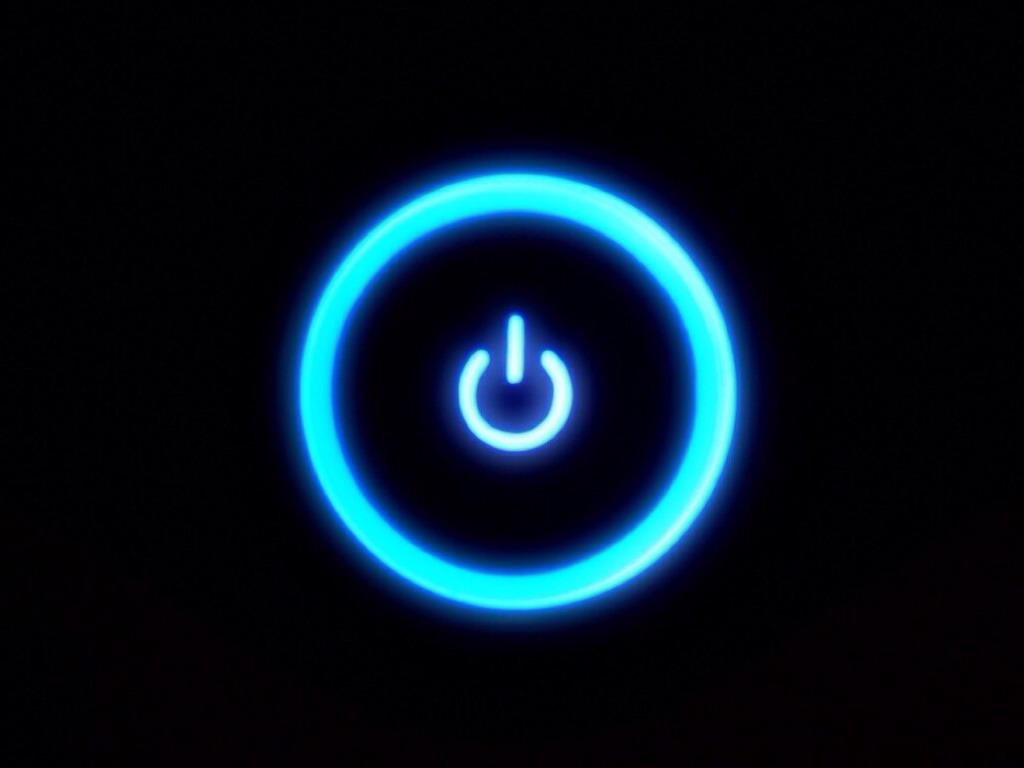
\includegraphics[scale=0.25]{switch.jpg}
\end{figure}
\end{frame}

\begin{frame}{Das BIOS tut seine Dinge}
\begin{figure}

\includegraphics[scale=0.25]{checking.jpg}
\end{figure}
\end{frame}

\begin{frame}{Master Boot Record (MBR) (x86)}
\Large
Erste Daten
\begin{itemize}
\item Ausführbarer code
\item Partitionen Table
\item Sucht Boot Partition
\end{itemize}
\end{frame}

\begin{frame}{Partition Boot Sector}
\Large
Erster und letzter Sektor
\begin{itemize}
\item Metadaten
\item BIOS Parameter block
\item Boot code
\end{itemize}
\end{frame}

\begin{frame}{BIOS parameter block (BPB)}
\begin{itemize}
\item Metadaten
\begin{itemize}
\item Sektoren pro Cluster
\item Bytes pro Sektor
\item ...
\end{itemize}
\item MFT Adresse
\end{itemize}
\end{frame}

\begin{frame}{Master File Table (MFT)}
\begin{figure}
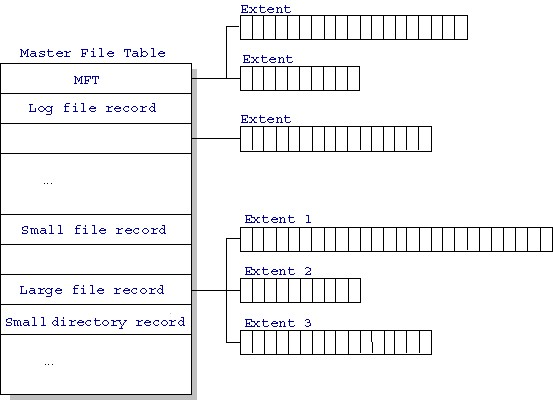
\includegraphics[scale=.7]{mft.jpg}
\end{figure}
\end{frame}

\begin{frame}{MFT}
\begin{itemize}
\item Kleine Dateien direkt in der MFT
\item Datei Attribute
\item Ordner werden in B-Trees angelegt
\end{itemize}
\end{frame}

\begin{frame}{Common Attributes}
\begin{columns}
\begin{column}{0.5\textwidth}
\large Table Attributes
\begin{itemize}
\item Time
\item Security
\end{itemize}
\end{column}
\begin{column}{0.5\textwidth}
\large File Attributes
\begin{itemize}
\item Hidden?
\item Compressed?
\end{itemize}
\end{column}
\end{columns}
\end{frame}

\begin{frame}{Compression}
\begin{itemize}
\item Drive/Folder/File
\item 4kb (cluster)
\item Integriert
\end{itemize}
\end{frame}

\begin{frame}{Encrypting File System (EFS)}

\end{frame}

\begin{frame}
\small
\begin{itemize}
\small
\item ntfs.com
\item docs.microsoft.com/en-us/windows-server/storage/file-server/ntfs-overview
\end{itemize}
\end{frame}

\end{document}